
\section{Experiments on hierarchical and grouped data}
\label{sec:experiments_on_hierarchical_and_grouped_data}

Our  research design\ref{fig:research_design} includes the following steps:
\begin{itemize}
    \item Data collection: identify datasets with hierarchical and grouped time series data describing sales/demand for multiple product categories and regions with exogenous variables.
    \item Tool evaluation: assess the applicability of existing libraries for hierarchical forecasting and XAI techniques.
    \item Model implementation: we build global models that consider multiple series and exogenous variables.
    \item Feature importance analysis: We apply model attribution methods and aggregation and decomposition techniques to identify key features and analyze their impact on the forecast.
    \item Model reasoning: analyze the feature contributions to forecast and identify underlying rules on different levels of the hierarchy.
\end{itemize}


\begin{figure}
    \centering
\begin{tikzpicture}[node distance=2cm]

%\node (start) [startstop] {Start};
\node (data) [process] {Data Collection};
\node (tool) [process, below of=data] {Tool Evaluation};
\node (model) [process, below of=tool] {Model Implementation};
\node (importance) [process, below of=model] {Feature Importance Analysis};
\node (reasoning) [process, below of=importance] {Model Reasoning};
%\node (stop) [startstop, below of=reasoning] {End};

%\draw [arrow] (start) -- (data);
\draw [->] (data) -- (tool);
\draw [->] (tool) -- (model);
\draw [->] (model) -- (importance);
\draw [->] (importance) -- (reasoning);
%\draw [arrow] (reasoning) -- (stop);

% Annotations
%\node [annotation, right=3cm of data.east, anchor=west] (dataann) {
%    \begin{itemize}
%        \item Find hierarchical time series data.
%        \item Include sales/demand across categories and regions.
%        \item Add relevant exogenous variables.
%    \end{itemize}
%};
%
%\node [annotation, right=3cm of model.east, anchor=west] (modelann) {
%    \begin{itemize}
%        \item Build global models for multiple time series.
%        \item Integrate exogenous variables.
%    \end{itemize}
%};
%
%\node [annotation, right=3cm of importance.east, anchor=west] (importanceann) {
%    \begin{itemize}
%        \item Determine feature importance.
%        \item Use aggregation and decomposition.
%        \item Assess feature impact on forecasts.
%    \end{itemize}
%};
%
%\node [annotation, right=3cm of reasoning.east, anchor=west] (reasoningann) {
%    \begin{itemize}
%        \item Analyze feature contributions.
%        \item Discover rules at different hierarchy levels.
%    \end{itemize}
%};
\end{tikzpicture}
\caption{Research design} \label{fig:research_design}
\end{figure}





\subsection{Datasets}
To model the hierarchical impact of features on forecasting, we must use datasets with multiple series and exogenous variables that represent demand drivers.
There are multiple open sales data sets available; however, there are just a few, such as the M5 competition~\citep{makridakis_m5_2022} and the Kaggle datasets~\citep{favorita-sales} that include exogenous variables.
For our initial exploration, we sampled M5 competition~\citep{makridakis_m5_2022} dataset, which includes sales data for multiple product categories and regions.
The dataset contains daily sales information for 3049 products in 10 stores over 5 years.
For our analysis, we identified three products that have similar sales patterns and are sold in two states and five stores.
As products are from the same category and department, the hierarchy at the product level was not considered.
The reason for this filtering is to reduce the complexity of the model and to focus on the feature importance analysis.
The selected products are FOODS\_3\_586, FOODS\_3\_080, and FOODS\_3\_555 and are sold in three states of Texas (TX), Wisconsin (WI).
The total sales data for these products are shown in Figure~\ref{fig:product_sales}.
Our hierarchical structure is shown in Figure~\ref{fig:hierarchical_structure}.
%It should be mentioned that the hierarchical structure can be inverted, meaning that the products can be at the top level and the stores at the bottom level, so technically our data set is grouped time series data.


\begin{figure}
    \centering
    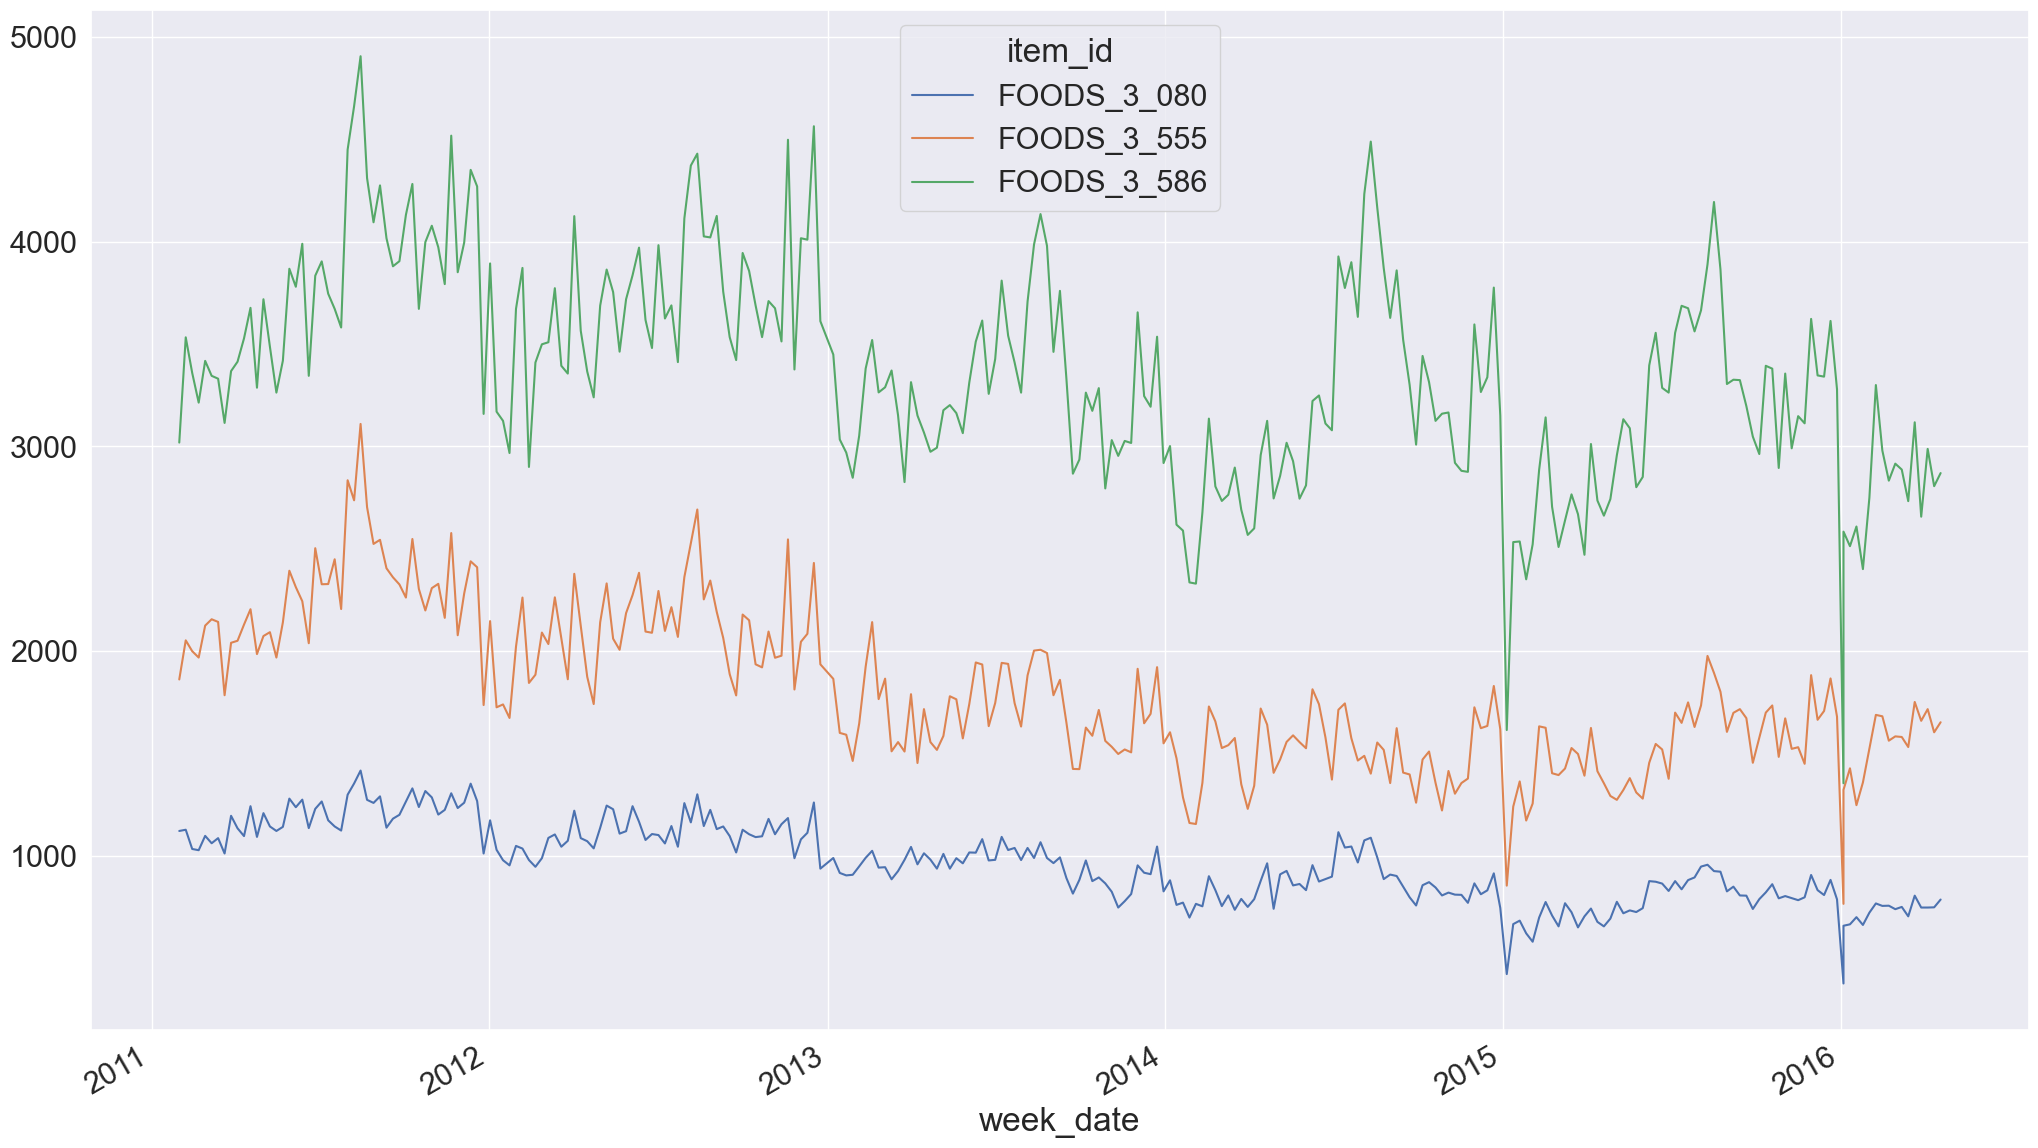
\includegraphics[width=0.8\linewidth]{chapters/05_feature_importance_hierarchy/img/product_sales }
    \centering
    \caption{Total weekly sales for the chosen products}
    \label{fig:product_sales}
\end{figure}


\begin{figure}
    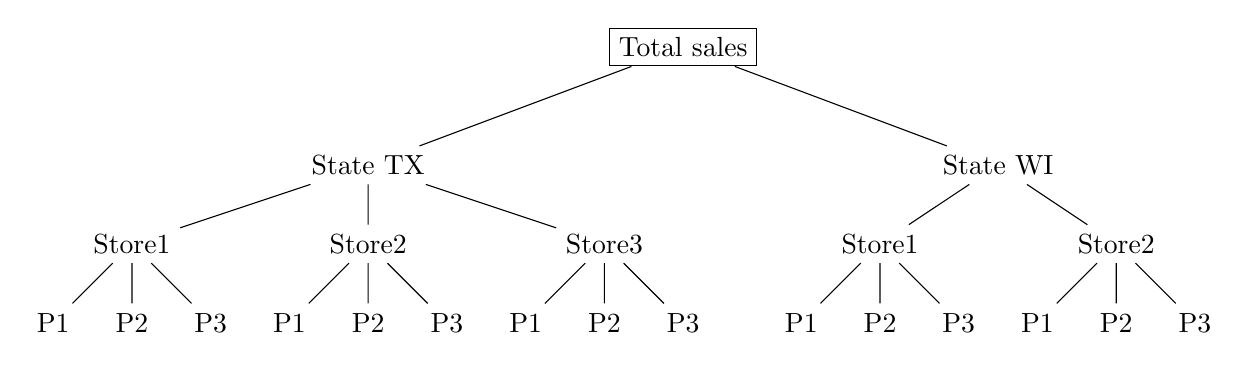
\begin{tikzpicture}
    [level 1/.style={sibling distance=80mm, level distance=15mm},
        level 2/.style={sibling distance=30mm, level distance=10mm},
        level 3/.style={sibling distance=10mm, level distance=10mm}]
        \node[rectangle,draw] {Total sales}
        child {node {State TX}
        child {node {Store1}
        child {node {P1}}
        child {node {P2}}
        child {node {P3}}
        }
        child {node {Store2}
        child {node {P1}}
        child {node {P2}}
        child {node {P3}}
        }
        child {node {Store3}
        child {node {P1}}
        child {node {P2}}
        child {node {P3}}
        }
        }
        child {node {State WI}
        child {node {Store1}
        child {node {P1}}
        child {node {P2}}
        child {node {P3}}
        }
        child {node {Store2}
        child {node {P1}}
        child {node {P2}}
        child {node {P3}}
        }
        };
    \end{tikzpicture}
    \caption{Hierarchical structure of product sales data (P1-3 = Product1-3)} \label{fig:hierarchical_structure}
\end{figure}




\subsection{Model implementation}\label{subsec:model-implementation}
The modelling approach is to build a single global on all series and exogenous variables for bottom-up aggregation.
For creating forecast models, the skforecast\cite{skforecast} library was used.
The base model for hierarchical forecasting was LightGBM~\cite{guolin_ke_highly_2017}
due to its efficiency and also because of its widespread usage in the M5 competition in this data set\cite{makridakis_m5_2022}.
Other ensemble models such as Random Forest or Gradient Boosting Machines could be used as well.
Other reasons for choosing LightGBM are that it can handle categorical variables without the need for one-hot encoding, and that it supports model-specific split and gain-based global feature importance methods.

Hyperparameter tuning was performed using the Optuna library\cite{optuna_2019}, by Bayesian optimisation.
The search space\ref{tab:hyperparam_search_space} was defined for the parameters of the LightGBM model, including the number of predictors, the minimum number of samples in the leaf, and the maximum depth of the tree.
In addition, the number of lagged sales records used as features was included in the search space.
For the search, the data was split into training and validation sets, the last year being the validation set used for backtesting.
The performance of the model was evaluated as a mean square error (MSE) in the validation set for each configuration.
The best configuration found was with 239 estimators and a maximum depth of 26 with a backtesting MSE 4263.01
The lagged sales records used as features were 1, 4, 5, 13, and 52 weeks.
\begin{table}
    \centering
    \begin{tabular}{|l|l|l|}
        \hline
        Parameter          & Search space & Description                                             \\
        \hline
        n\_estimators      & 50-1000      & Number of boosting iterations                           \\
        max\_depth         & 5-50         & Maximum depth of the tree                               \\
        min\_samples\_leaf & 1-10         & Minimum number of samples required to be at a leaf node \\
        num\_lagged\_sales & 4-52         & Number of lagged sales records used as features         \\
        \hline
    \end{tabular}
    \caption{Model hyperparameters search space}
    \label{tab:hyperparam_search_space}
\end{table}

The feature input for the final model is a table with the following columns:
\begin{itemize}
    \item week\_of\_year represented as numerical values (1-52)
    \item sell\_price for the week for the product in the store
    \item num\_of\_events for the week
    \item snap\_days for the week in the state
    \item lag\_\emph{n} for n in [1, 4, 5, 13, 52] representing the sales from the previous weeks
    \item series\_id noted as (\_level\_skforecast) encoded as a numerical value representing the series hierarchy
\end{itemize}
%\emph{Series\_id} could have been encoded as a one-hot encoded vector or as a categorical variable given it is supported by LightGBM.
%One-hot encoded vector would have increased the number of features and the complexity of the model,
%while with the categorical variable, the model would have been able to learn the hierarchy structure.